\section{Evaluation}

\subsection{LP Solver scalability}
\begin{alltt}\scriptsize
# of attrbutes vs solving time:
\end{alltt}

\begin{figure}[t]
\centerline{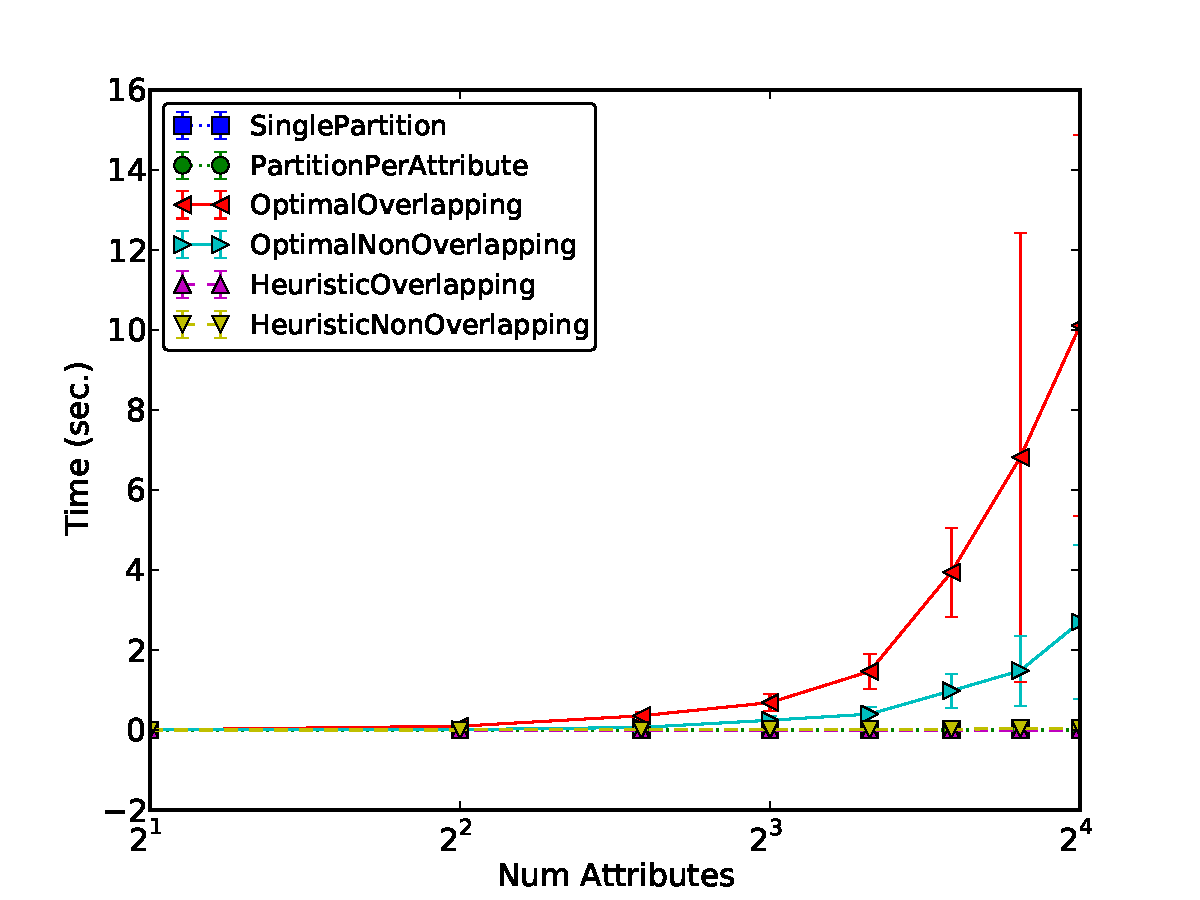
\includegraphics[width=0.9\columnwidth]{figures/RunningTimeVsNumAttributes.pdf}}
\caption{The running time for different solvers as the number of attributes increases.}
\end{figure}



\subsection{I/O comparison}

\begin{figure}[t]
\centerline{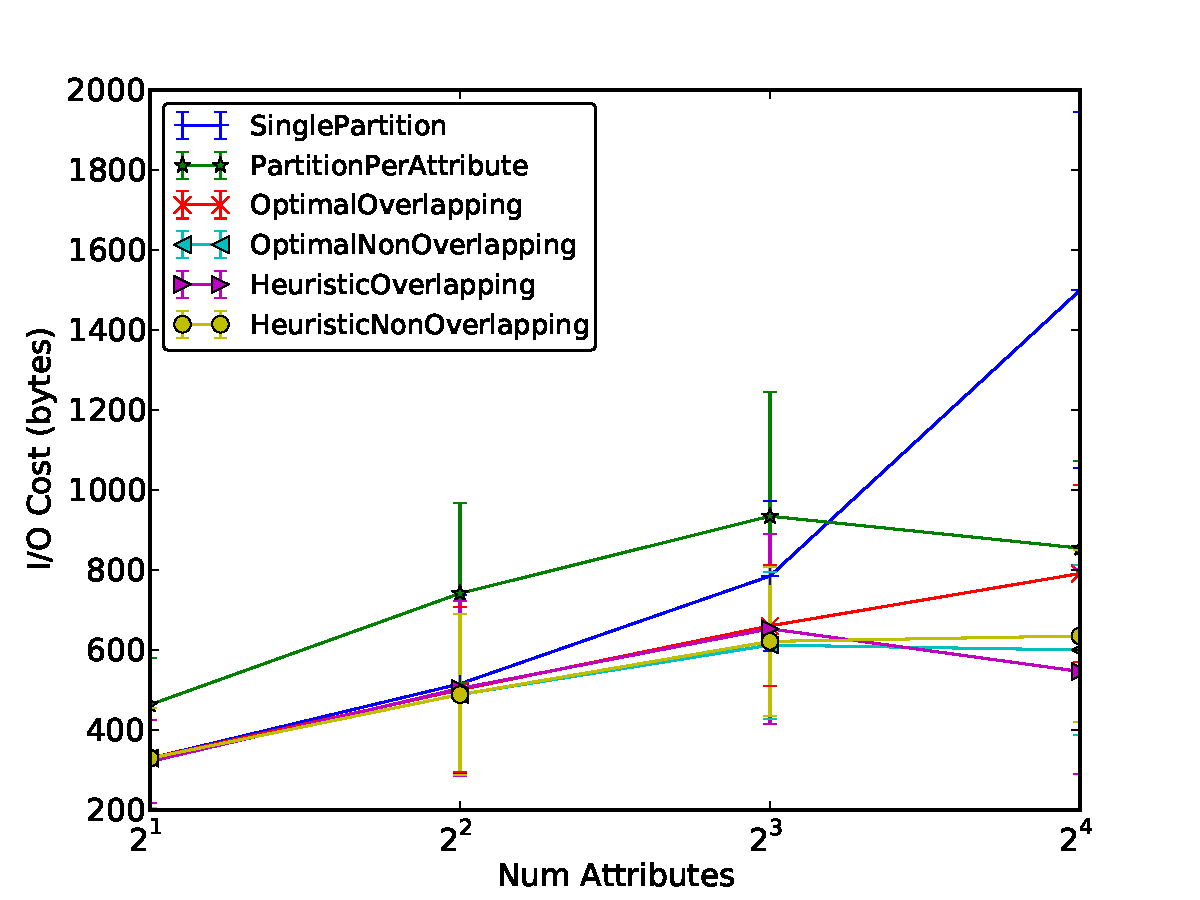
\includegraphics[width=0.9\columnwidth]{figures/QueryIOVsNumAttributes.pdf}}
\caption{The query I/O cost for different solvers as the number of attributes increases.}
\end{figure}


\begin{figure}[t]
\centerline{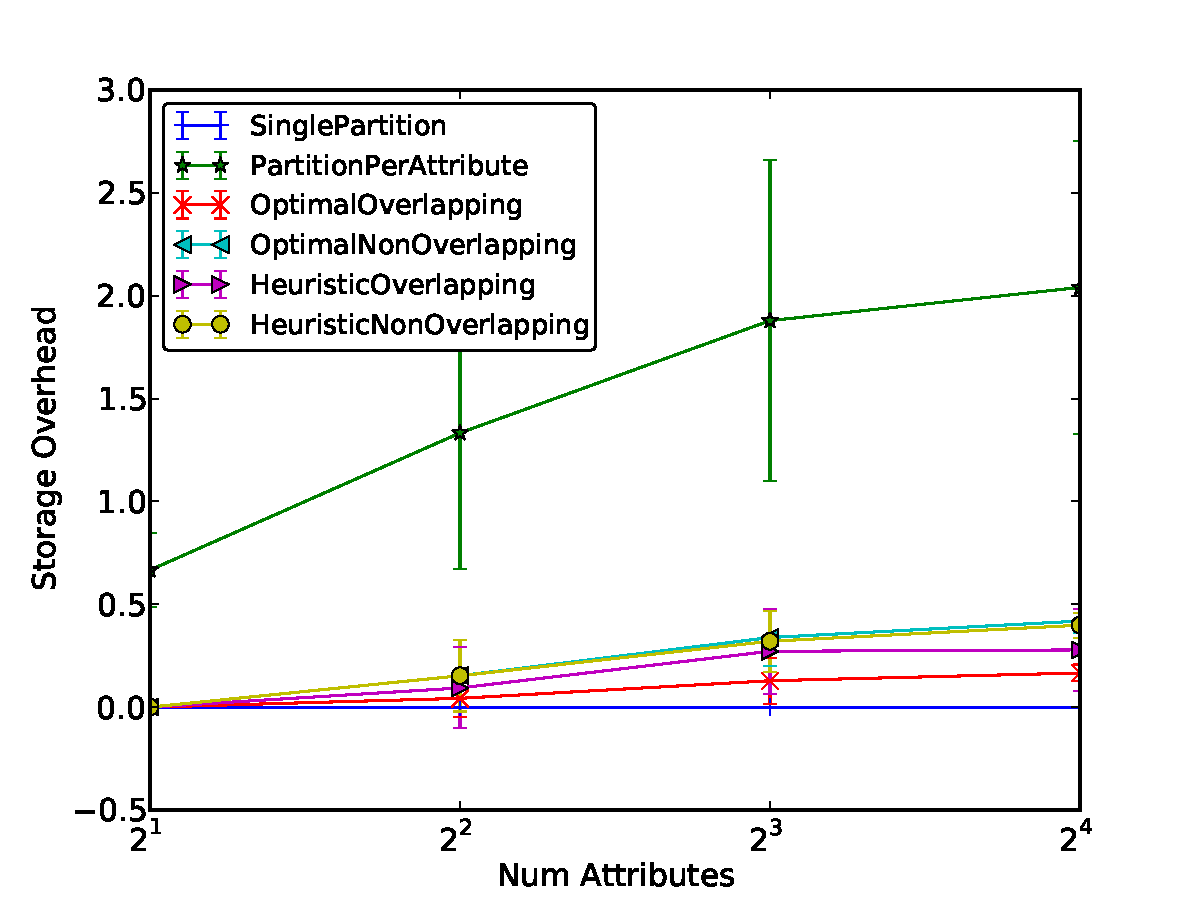
\includegraphics[width=0.9\columnwidth]{figures/StorageOverheadVsNumAttributes.pdf}}
\caption{The storage overhead for different solvers as the number of attributes increases.}
\end{figure}



\begin{verbatim}
1) RunningTimeVsNumAttributes:
  x axis: # attributes
  y axis: running time
  series: optimal-nov, optimal-ov, heuristic-nov, heuristic-ov

2) RunningTimeVsNumQueryKinds:
  x axis: num query kinds
  y axis: running time
  series: optimal-nov, optimal-ov, heuristic-nov, heuristic-ov

3) QueryIOVsNumAttributes:
  x axis: # attributes
  y axis: query IO
  series: optimal-nov, optimal-ov, heuristic-nov, heuristic-ov, single-block, per-attribute

4) StorageOverheadVsNumAttributes:
  x axis: # attributes
  y axis: storage overhead
  series: optimal-nov, optimal-ov, heuristic-nov, heuristic-ov, single-block, per-attribute
  
5) QueryIOVsStorageOverheadThreshold:
  x axis: query overhead threshold
  y axis: query IO
  series: optimal-nov, optimal-ov, heuristic-nov, heuristic-ov, single-block, per-attribute

6) StorageOverheadVsStorageOverheadThreshold:
  x axis: query overhead threshold
  y axis: storage overhead
  series: optimal-nov, optimal-ov, heuristic-nov, heuristic-ov, single-block, per-attribute

7) QueryIOVsNumQueryKinds:
  x axis: num query kinds
  y axis: query IO
  series: optimal-nov, optimal-ov, heuristic-nov, heuristic-ov, single-block, per-attribute

8) StorageOverheadVsNumQueryKinds:
  x axis: num query kinds
  y axis: storage overhead
  series: optimal-nov, optimal-ov, heuristic-nov, heuristic-ov, single-block, per-attribute

9) QueryIOVsAttributeSizeSkew:
  x axis: attribute size skew
  y axis: query IO
  series: optimal-nov, optimal-ov, heuristic-nov, heuristic-ov, single-block, per-attribute

10) StorageOverheadVsAttributeSizeSkew:
  x axis: attribute size skew
  y axis: storage overhead
  series: optimal-nov, optimal-ov, heuristic-nov, heuristic-ov, single-block, per-attribute

11) QueryIOVsQueryLength:
  x axis: mean query length
  y axis: query IO
  series: optimal-nov, optimal-ov, heuristic-nov, heuristic-ov, single-block, per-attribute

12) StorageOverheadVsQueryLength:
  x axis: mean query length
  y axis: storage overhead
  series: optimal-nov, optimal-ov, heuristic-nov, heuristic-ov, single-block, per-attribute

13) QueryIOVsQueryFreqSkew:
  x axis: query freq skew
  y axis: query IO
  series: optimal-nov, optimal-ov, heuristic-nov, heuristic-ov, single-block, per-attribute

14) StorageOverheadVsQueryFreqSkew:
  x axis: query freq skew
  y axis: storage overhead
  series: optimal-nov, optimal-ov, heuristic-nov, heuristic-ov, single-block, per-attribute
\end{verbatim}

